\begin{enumerate}[(a)]
\item \begin{table}[ht]
\caption{Empirical survival estimate by hand.}
% title of Table
\centering
% used for centering table
\begin{tabular}{c c c}
% centered columns (4 columns)
\hline
\hline
   Time & failures & $S(t^{+})$  \\ \hline
     1  &      1 & 11/12 = 0.917 \\
     2  &      3 & 8/12 = 0.667 \\
     3  &      1 & 7/12 = 0.583 \\ 
     5  &      1 & 6/12 = 0.500 \\
     6  &      1 & 5/12 = 0.417 \\
     7  &      1 & 4/12 = 0.333 \\ 
     8  &      1 & 3/12 = 0.250 \\ 
    16  &      1 & 2/12 = 0.167 \\ 
    17  &      1 & 1/12 = 0.083 \\ 
    34  &      1 & 0/12 = 0.000 \\
\hline
\end{tabular}
\label{table:1}
\end{table}
We first create a vector (i.e., a series of numbers) of the survival times using the function \verb|c|. Then, we create a data frame containing the distinct survival times along with the number of failures at each time point. The name of the first column is \emph{time}, while the name of the second one is \emph{failures}. Please, note that the function \verb|unique| removes the duplicate elements of its input, and the function \verb|table| returns a frequency table (very similar to the \verb|STATA| command \verb|tabulate|).
Using \verb|R| code,
\begin{footnotesize}
\begin{verbatim}
> # (a)
> # Time to death or relapse
> time = c(1,2,2,2,3,5,6,7,8,16,17,34)
> 
> # Create a data frame with the survival time, 
> # the number of deaths at each time point (assuming no censoring)
> # and the empirical survival estimate
> surv.table = data.frame(time = unique(time), failures = c(table(time)) )
> 
> # Number of patients being alive
> surv.table$alive = 12 - cumsum(surv.table$failures)
> 
> # Survival probability
> surv.table$surv = surv.table$alive/12
> surv.table
   time failures alive       surv
1     1        1    11 0.91666667
2     2        3     8 0.66666667
3     3        1     7 0.58333333
5     5        1     6 0.50000000
6     6        1     5 0.41666667
7     7        1     4 0.33333333
8     8        1     3 0.25000000
16   16        1     2 0.16666667
17   17        1     1 0.08333333
34   34        1     0 0.00000000
\end{verbatim}
\end{footnotesize}
\item First, a data frame with the survival times and the failure indicator (a column of ones, since we assume that there is no censoring at this stage) is created.
Through the \verb|Surv| function we declare that we have survival data. The first argument is the survival time while the second argument is the failure indicator.
 Then, the \verb|survfit| can be used to get the empirical survival estimates. The details of the estimation are available by the \verb|summary| function.
\begin{footnotesize}
\begin{verbatim}
> # (b)
> # Don't forget to import library survival
> library(survival)
Loading required package: splines
> nhl.data = data.frame(time = time, delta = 1)
> 
> # Use the Surv function to declare survival data
> nhl.fit = survfit(Surv(time,delta) ~ 1,data = nhl.data)
> summary(nhl.fit)
Call: survfit(formula = Surv(time, delta) ~ 1, data = nhl.data)

 time n.risk n.event survival std.err lower 95% CI upper 95% CI
    1     12       1   0.9167  0.0798       0.7729        1.000
    2     11       3   0.6667  0.1361       0.4468        0.995
    3      8       1   0.5833  0.1423       0.3616        0.941
    5      7       1   0.5000  0.1443       0.2840        0.880
    6      6       1   0.4167  0.1423       0.2133        0.814
    7      5       1   0.3333  0.1361       0.1498        0.742
    8      4       1   0.2500  0.1250       0.0938        0.666
   16      3       1   0.1667  0.1076       0.0470        0.591
   17      2       1   0.0833  0.0798       0.0128        0.544
   34      1       1   0.0000     NaN           NA           NA
\end{verbatim}
\end{footnotesize}
\item The \verb|plot| function produces a graph of the estimated survival function when taking an object created by \verb|survfit| as an argument. We set the working directory through the function \verb|setwd|. There are plenty of ways to save a graph in \verb|R| (for example, see ?png). To save your graph in a pdf format, just use the \verb|pdf| function before the \verb|plot| function and type \verb|dev.off()| after it. 
\begin{footnotesize}
\begin{verbatim}
# (c)
# Set working directory
setwd("C:/Applied_Survival_Analysis_Jan2016/lab1/graphs")

pdf('lab1EmpSurv.pdf',width = 5,height = 5)
plot(nhl.fit,conf.int = F,mark.time = F,xlab = "Time to death or relapse",
     ylab = "Survival probability")
dev.off()
\end{verbatim}
\end{footnotesize}
\begin{figure}[htbp]
	\centering
		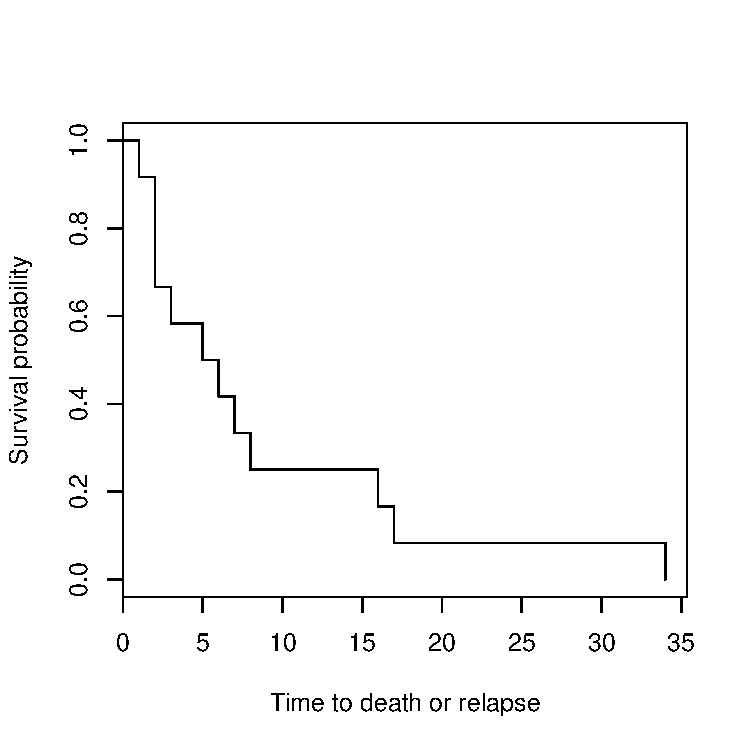
\includegraphics[]{lab1EmpSurv.pdf}
		%\rule{35em}{0.5pt}
	\caption{Estimated survival probability for 12 patients
with non-Hodgkin’s lymphoma.}
	\label{figure1}
\end{figure}
\item It is assumed that the probability of an event (relapse or death) is a binomial 
proportion. Thus, the probability of relapse or death at time $t=6^+$
is $p=x/n = 7/12 = 0.583$, or, $S(6^{+}) = 5/12 = 0.417$. According to the standard error of the binomial distribution, we get
\begin{align}
se = \sqrt{\dfrac{p(1-p)}{n}} = \sqrt{\dfrac{0.583(1-0.417)}{12}} = 0.1423,
\nonumber
\end{align}
and using \verb|R| code
\begin{footnotesize}
\begin{verbatim}
> # (d)
> # Calculation of standard errors
> # Just the SE of a binomial proportion, p(1-p)/n
> surv.table$se = sqrt(surv.table$surv*(1-surv.table$surv)/12)
> surv.table[,c("time","se")]
   time         se
1     1 0.07978559
2     2 0.13608276
3     3 0.14231876
5     5 0.14433757
6     6 0.14231876
7     7 0.13608276
8     8 0.12500000
16   16 0.10758287
17   17 0.07978559
34   34 0.00000000
\end{verbatim}
\end{footnotesize}
\item The \textbf{median} survival time is the smallest time, $\tau$, such that
$S(\tau^{+})\leq 0.5$, so the estimated median is 5. \\
\textbf{Lower quartile (25\%):} the smallest time ($LQ$) such that
$S(LQ^{+})\leq 0.75$. Since $S(2^{+}) = 0.667$, the estimated 25\%-ile time is 2. \\
\textbf{Upper quartile (75\%):} the smallest time ($UQ$) such that 
$S(UQ^{+})\leq 0.25$. Since $S(8^{+}) = 0.250$, the estimated 75\%-ile time is 8. To get the above information in \verb|R|, use the \verb|quantile| function
\begin{footnotesize}
\begin{verbatim}
> # (e)
> # Median survival
> quantile(nhl.fit,probs = c(0.25,0.50,0.75),conf.int = F)
  25   50   75 
 2.0  5.5 12.0 
\end{verbatim}
\end{footnotesize}
It seems that \verb|R| uses a slightly different algorithm to determine the quartiles. However, this would be of minor importance if the sample size was large.
\end{enumerate}
